\documentclass[a4paper]{article}
\usepackage[a4paper, top=17mm, bottom=17mm, left=17mm, right=17mm]{geometry}
\usepackage[utf8]{inputenc}
\usepackage[T2A,T1]{fontenc}
\usepackage[colorlinks,filecolor=blue,citecolor=green,unicode,pdftex]{hyperref}
\usepackage{cmap}
\usepackage[english,russian]{babel}
\usepackage{amsmath}
\usepackage{amssymb,amsfonts,textcomp}
\usepackage{color}
\usepackage{array}
\usepackage{hhline}
\hypersetup{colorlinks=true, linkcolor=blue, citecolor=blue, filecolor=blue, urlcolor=blue, pdftitle=1, pdfauthor=, pdfsubject=, pdfkeywords=}
% \usepackage[pdftex]{graphicx}
\usepackage{graphicx}
% \usepackage{epigraph}
% Раскомментировать тем, у кого этот пакет есть. Шрифт станет заметно красивее.
%\usepackage{literat}
\usepackage{indentfirst}
\usepackage{wrapfig}

\sloppy
\pagestyle{plain}
%\pagestyle{empty}

\title{Метамоделирование: современный подход к созданию средств визуального проектирования}

\author{А.С. Кузенкова \and Ю.В. Литвинов \and Т.А. Брыксин}
\date{}
\begin{document}

\maketitle
\thispagestyle{empty}

\begin{quote}
\small\noindent
В статье описывается реализация поддержки метапрограммирования в системе QReal. Приводится краткое описание архитектуры системы, процесса создания нового визуального языка метасредствами системы, в том числе приводится описание визуального метаредактора и механизмов интеграции метаредактора в среду.
\end{quote}

\section*{Введение}
В настоящее время средства визуального моделирования активно используются для разработки программного обеспечения. Некоторые инструментарии не ориентированы на конкретную предметную область и имеют заранее определенный набор редакторов визуальных языков для создания новых систем. Такие инструментарии называются CASE-пакетами. Их использование само по себе может значительно упростить проектирование сложных систем по сравнению с подходами, основанными на использовании текстовых языков. Но иногда процесс разработки можно упростить ещё более --- к примеру, если система проектируется для узко специализированной предметной области, её создание с применением описанного подхода может стать неоправданно трудоёмким. В этом случае уместен другой способ разработки новых систем --- предметно-орентированное моделирование~\cite{theBook}. Суть его состоит в том, что вместо использования уже имеющихся визуальных языков создается новый язык, специализированный для рассматриваемой предметной области, и система проектируется уже с помощью разработанного языка. Как показывает практика, такой подход является более гибким и удобным~\cite{kieburtz}.

Примерами средств для создания новых предметно-ориентированных языков, или DSL (Domain Specific Languages), являются Microsoft DSL Tools\footnote{http://msdn.microsoft.com/en-us/library/bb126259.aspx}, Eclipse GMF\footnote{www.eclipse.org/gmf/}, MetaEdit+\footnote{http://www.metacase.com}.

Инструментарий Microsoft DSL Tools используется для создания редакторов визуальных языков, встроенных в среду Visual Studio, и хорошо применим для создания несложных графических редакторов. Создание нового графического редактора состоит в описании его метамодели с возможностью дополнения требуемой функциональности на C\#. Но с помощью него нельзя создать редактор визуального языка, независимый от среды Microsoft Visual Studio.

Технология Eclipse GMF разрабатывается на базе среды разработки Eclipse и также предназначена для создания новых предметно-ориентированных языков, в основном встроенных в эту среду. Но для создания метамодели языка, в свою очередь, требуется описание нескольких моделей (доменной, графической модели, моделей инструментов, соответствия и генератора), поэтому процесс создания нового языка оказывается довольно длительным и трудоёмким.

MetaEdit+ является развитым инструментарием для создания DSM-решений, имеет большое число промышленных внедрений, но цена лицензии на него весьма высока.

Нашей целью была разработка инструментария, сочетающего в себе преимущества существующих и, по возможности, лишенного их недостатков.

\section{QReal}

На кафедре системного программирования СПбГУ в течение нескольких лет разрабатывается среда визуального программирования QReal~\cite{qReal}. Изначально ставилась задача поддержки языка UML 2~\footnote{http://uml.org/} и уже на самых ранних этапах разработки стало ясно, что реализация всех 13 видов диаграмм UML ручным кодированием потребует неоправданно больших усилий. Была разработана следующая схема для упрощения труда программистов: каждая диаграмма языка описывалась на специальном метаязыке (аналогичном языку MOF, который используется для задания метамодели UML), по XML-файлам с такими описаниями генерировался код на C++, который потом собирался в динамическую библиотеку и подключался к основной части системы как плагин. Такая схема показала себя довольно удобной и позволила задавать не только диаграммы UML, но и описывать другие существующие визуальные языки с графовой структурой, например, BPEL~\footnote{http://www.ibm.com/developerworks/library/specification/ws-bpel/}. Также оказалось возможным создавать новые визуальные языки и генерировать для них инструментальную поддержку. 

Общая архитектура системы показана на рисунке~\ref{architecture}. Вся информация о синтаксисе языка хранится в плагине, а основная часть системы работает в терминах, общих для всех языков. Создаваемые в QReal модели хранится в репозитории, который также не использует информацию о синтаксисе конкретных языков, с помощью которых эти модели были разработаны.

\begin{figure}[ht]
  \begin{center}
    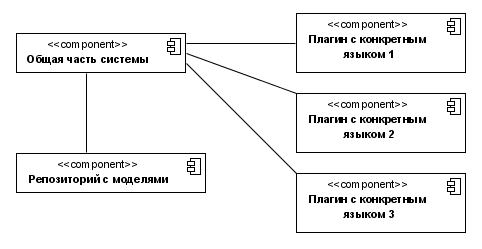
\includegraphics[width=0.5\textwidth]{architecture.jpg}
    \caption{Общая архитектура QReal}
    \label{architecture}
  \end{center}
\end{figure}

Добавление нового визуального языка в QReal состоит из следующих этапов: абстрактный и конкретный синтаксис языка описывается с помощью метаязыка в XML файле. Из него автоматически генерируется код на C++, реализующий специфику конкретных редакторов и использующий интерфейсы, объявленные в основной части системы. Сгенерированный код компилируется в динамическую библиотеку, которая при запуске грузится основной частью.

Такой способ создания новых графических редакторов, хотя и оказался удобным в работе и более эффективным по сравнению с ручным кодированием, но всё же имеет ряд принципиальных недостатков. Во-первых, написание XML-файла --- это довольно кропотливый процесс, поскольку описание каждого элемента громоздко и не наглядно. Во-вторых, пользователю необходимо обладать определенными знаниями касаемо строения метаметамодели языка и навыками работы с XML.

\section{Метаредактор}

Заметим, что XML-описания редакторов можно генерировать по визуальным моделям, тем самым применив технологию предметно-ориентированной разработки саму к себе.

\begin{figure}[ht]
  \begin{center}
    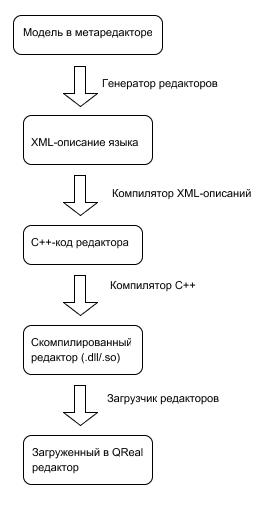
\includegraphics[width=0.25\textwidth]{editorGeneration.jpg}
    \caption{Процесс генерации редактора}
    \label{editorGeneration}
  \end{center}
\end{figure}

В связи с этим в QReal были добавлены визуальные инструменты поддержки метамоделирования. Для этих целей был разработан специальный визуальный язык для создания других визуальных языков (или метаязык), базовыми абстракциями которого являются сущности и отношения. Был создан реализующий его графический редактор (или метаредактор). Рассмотрим метаязык и метаредактор подробнее. 

Подключаемый модуль может содержать несколько визуальных языков. Каждый язык определяется набором своих элементов и связей между ними. Основные абстракции делятся на графические и неграфические (соответственно имеющие и не имеющие графического представления в редакторе). В метаредакторе графическими являются такие сущности, как ``Элемент''  и ``Связь'', обозначающие, соответственно, элемент визуального языка и связь между элементами. Примером неграфической сущности является ``Перечислимый тип данных'' (enum), обозначающая перечень значений, которые могут использоваться для указания свойств элементов. Также с помощью метаредактора можно задавать отношения наследования между элементами на диаграмме и отношения допустимой вложенности одних элементов в другие. Эти отношения на диаграмме указываются стрелками. Помимо этого имеется возможность задавать некоторые дополнительные свойства, поддержка которых осуществлена в QReal (способность “вытягивать” из элементов определенные связи, сортировать вложенные элементы и уметь их скрывать для элементов-контейнеров, и другое). 

В QReal для разработанного метаязыка была создана инструментальная поддержка и соответствующая инфраструктура. После построения метамодели (или нескольких метамоделей) языка пользователь имеет возможность конвертировать его в используемый XML-формат. Инфраструктура обеспечивает поддержку сквозного процесса создания графических редакторов. С ее помощью разработчик может спроектировать новый визуальный язык, скомпилировать подключаемый модуль соответствующего графического редактора и подключить его к QReal, не выходя из системы. Кроме этого реализован разбор существующих XML-файлов и их визуализация с помощью метаредактора, тем самым помимо создания новых визуальных языков пользователь может редактировать уже имеющиеся. Таким образом, парсер XML-файлов совместно с генератором в XML-формат обеспечивают совместимость двух используемых в QReal способов задания метамоделей --- в текстовом и графическом виде.

Процесс разработки графического редактора начинается с создания элемента, обозначающего сам редактор. В свойствах элемента указывается его название и имя директории, в которой будет сохранен код сгенерированного редактора. Далее создаются диаграммы языков, внутри каждой диаграммы задается метамодель соответствующего языка. У каждого элемента указываются логическое имя, с которым работают генераторы и интерпретаторы моделей, и видимое имя, которое показывается пользователю. Эти имена можно устанавливать взаимонезависимо. Для элементов указываются логические свойства, которые потом можно редактировать в процессе разработки моделей на этом языке, и они используются для генерации или интерпретации моделей. Задаются отношения наследования и вложенности, указываются дополнительные свойства, которыми обладают элементы. Когда проектирование редактора завершено, пользователь может сразу сгенерировать редактор. Если имеются ошибки в задании метамодели (к примеру, не указаны необходимые свойства элементов), то сообщения о них появятся в специальном окне, и имеется возможность их исправить. Если же всё сделано правильно, пользователю предлагается сразу подключить редактор к среде.  

Процесс сборки нового языка в QReal схематически изображён на рисунке~\ref{editorGeneration}

\section{Заключение}
Описанный в статье метаредактор реализован и используется в системе QReal для создания новых визуальных языков. Один из примеров языка, разработанного с помощью метаредактора --- язык программирования роботов Lego Mindstorms NXT\footnote{http://mindstorms.lego.com}. Этот визуальный язык позволяет задавать логику поведения робота в виде последовательности управляющих блоков, таких как ``Включить мотор на таком-то порту с такой-то мощностью'', и исполнить программу на роботе, интерпретируя диаграмму и посылая команды роботу через Bluetooth. Визуальный язык прост и понятен, что даёт возможность его использовать даже ученикам начальной школы. Пример диаграммы на этом языке изображён на рисунке~\ref{robotsDiagram}. Метамодель этого языка несложная, добавить новый элемент в язык чрезвычайно просто --- перетащить элемент с палитры, задать его свойства, нарисовать в редакторе его внешний вид, сгенерировать редактор и тут же начать новый элемент использовать. Создание редактора этого языка с помощью метаредактора заняло порядка нескольких часов, причем большую часть заняло создание внешних представлений элементов на диаграммах. Для сравнения, ручное кодирование такого редактора даже при наличии соответствующей инфраструктуры, оценивается в несколько человеко-месяцев.

\begin{figure} [ht]
  \begin{center}
    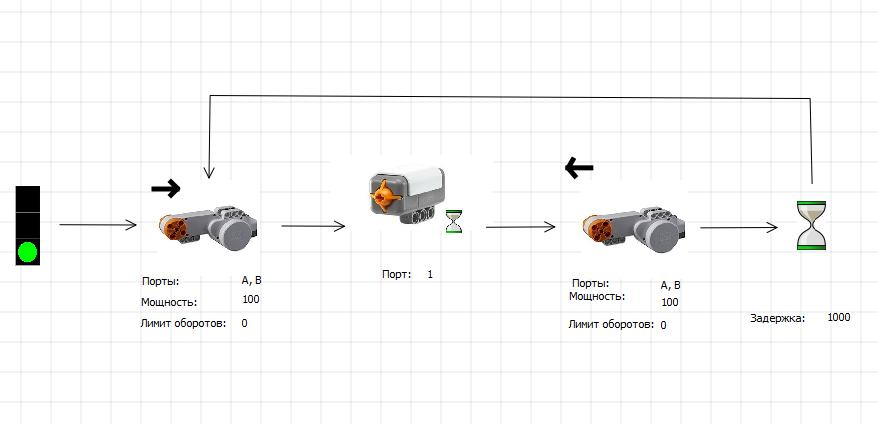
\includegraphics[width=0.8\textwidth]{robotsDiagram.jpg}
    \caption{Диаграмма поведения робота}
    \label{robotsDiagram}
  \end{center}
\end{figure}

%\begin{figure} [ht]
%  \begin{center}
%    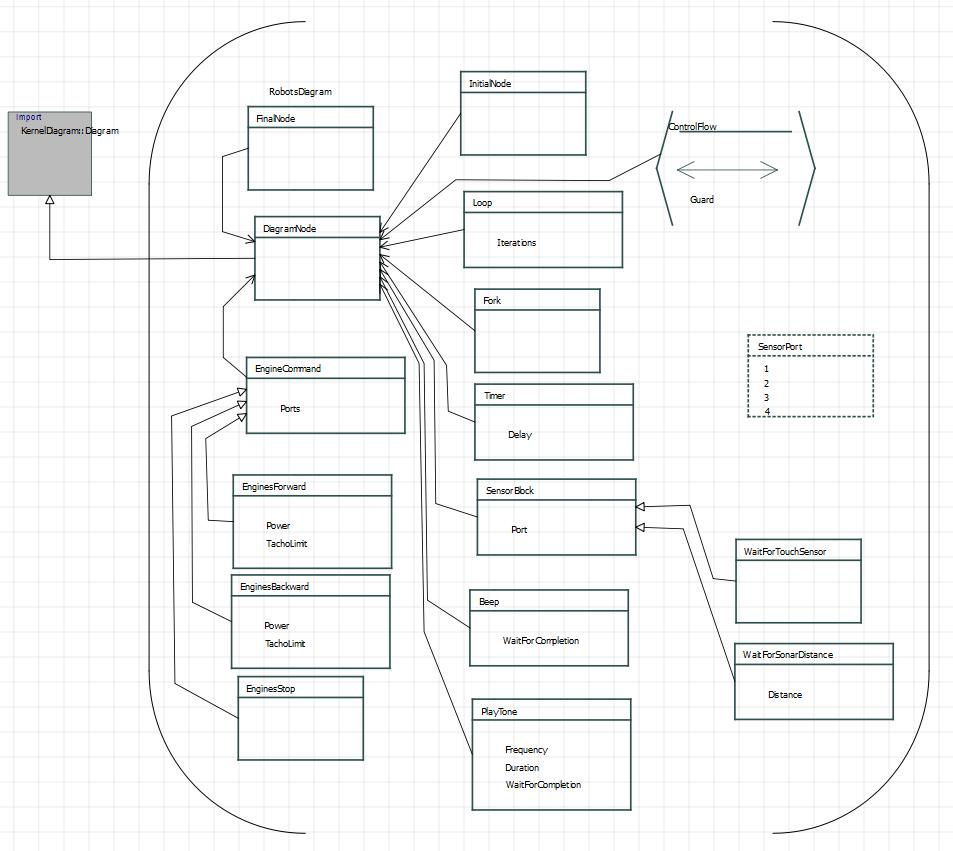
\includegraphics[width=0.6\textwidth]{robotsMetamodel.jpg}
%    \caption{Метамодель редактора диаграмм роботов}
%    \label{robotsMetamodel}
%  \end{center}
%\end{figure}

\begin{thebibliography}{9001}
  \bibitem{qReal} А.Н. Терехов, Т.А. Брыксин, Ю.В. Литвинов и др., Архитектура среды визуального моделирования QReal. // Системное программирование. Вып. 4. СПб.: Изд-во СПбГУ. 2009, С. 171-196
	\bibitem{kieburtz} Kieburtz, R., et al. A software engineering experiment in software component generation, Proceedings of 18th International Conference on Software Engineering, Berlin, IEEE Computer Society Press, March, 1996
  \bibitem{theBook} Kelly, S., Tolvanen, J. Domain-Specific Modeling: Enabling Full Code Generation // Wiley-IEEE Computer Society Press. 2008. 448 pp.
\end{thebibliography}

\end{document}